\documentclass[9pt]{beamer}
\usetheme{cmepda}

\usepackage[utf8]{inputenc}
\usepackage[T1]{fontenc}

\graphicspath{{figures/}} 


\title{OOP introduction (1/2)}
\subtitle{Computing Methods for Experimental Physics and Data Analysis}
\date{Compiled on \today}
\author{A. Manfreda}
\institute[INFN]{INFN--Pisa}
\email{alberto.manfreda@pi.infn.it}


\begin{document}


\titleframe


\begin{frame}
  \frametitle{Smart variables}
  
  \begin{itemize}
    \item Working with containers like lists or dictionaries, you may have noticed
          that they can do many thing besides holding the data
    \medskip
    \begin{itemize}
      \item You can extend a list using append() or insert()
      \item Trying to access a non-existent index in a list triggers a specific error (\emph{IndexError})
      \item You can iterate on a list using the handy for-loop Python syntax
      \item and so on\dots
     \end{itemize}
     \medskip
     \item In other words, a list is a variable that, in addition to its data,
           shows some kind of specific \emph{behaviour}.
     \medskip
     \item How is that implemented?
  \end{itemize}
\end{frame}



\begin{frame}
  \frametitle{Object Oriented Programming (OOP)}
  
  \begin{itemize}
    \small
    \item Programming paradigm based on \emph{objects}
    \bigskip
    \item An object is a code entity that has:
    \smallskip
    \begin{itemize}
      \item \alert{State} $\rightarrow$ data (usually called \emph{member variables} or \emph{attributes})
      \smallskip
      \item \alert{Behaviour} $\rightarrow$ functions (usually called \emph{member functions} or \emph{methods})
    \end{itemize}
    \bigskip
    \item The idea is: keep together the variables and the code that manipulates them
    \bigskip
    \item As the name suggests, OOP is very often adopted for modeling systems that are naturally
          described in terms of objects  
    \begin{itemize}
      \smallskip
      \item Physical simulations
      \smallskip
      \item Graphical engines
      \smallskip
      \item Graphical User Interfaces (GUI) 
    \end{itemize}

  \end{itemize}
\end{frame}


\begin{frame}
  \frametitle{Why should I care?}
  
  \begin{itemize}
    \item Object-oriented programming is one of the most widely used paradigm today
    \smallskip
    \item That doesn't necessarily mean it is the best one -- nor the right tool for any job \\
    \tiny
    \url{https://en.wikipedia.org/wiki/Object-oriented_programming\#Criticism}
    \normalsize
    \smallskip
        
    \item There is a number of famous programmers which really dislike it (e.g. \emph{Linus Torvalds})
    \medskip
    \item Still, it is something you definitely want in your toolbox
    \medskip
    \item And there is a fairly good chance that you will have to interact with some OOP
          code in your life
    \smallskip   
  \end{itemize}

\end{frame}


\begin{frame}
  \frametitle{A good reason for learning OOP}
  
  \begin{itemize}
    \item (Almost) every popular languages nowadays is OO
  \end{itemize}
  
  \smallskip
  
  \centering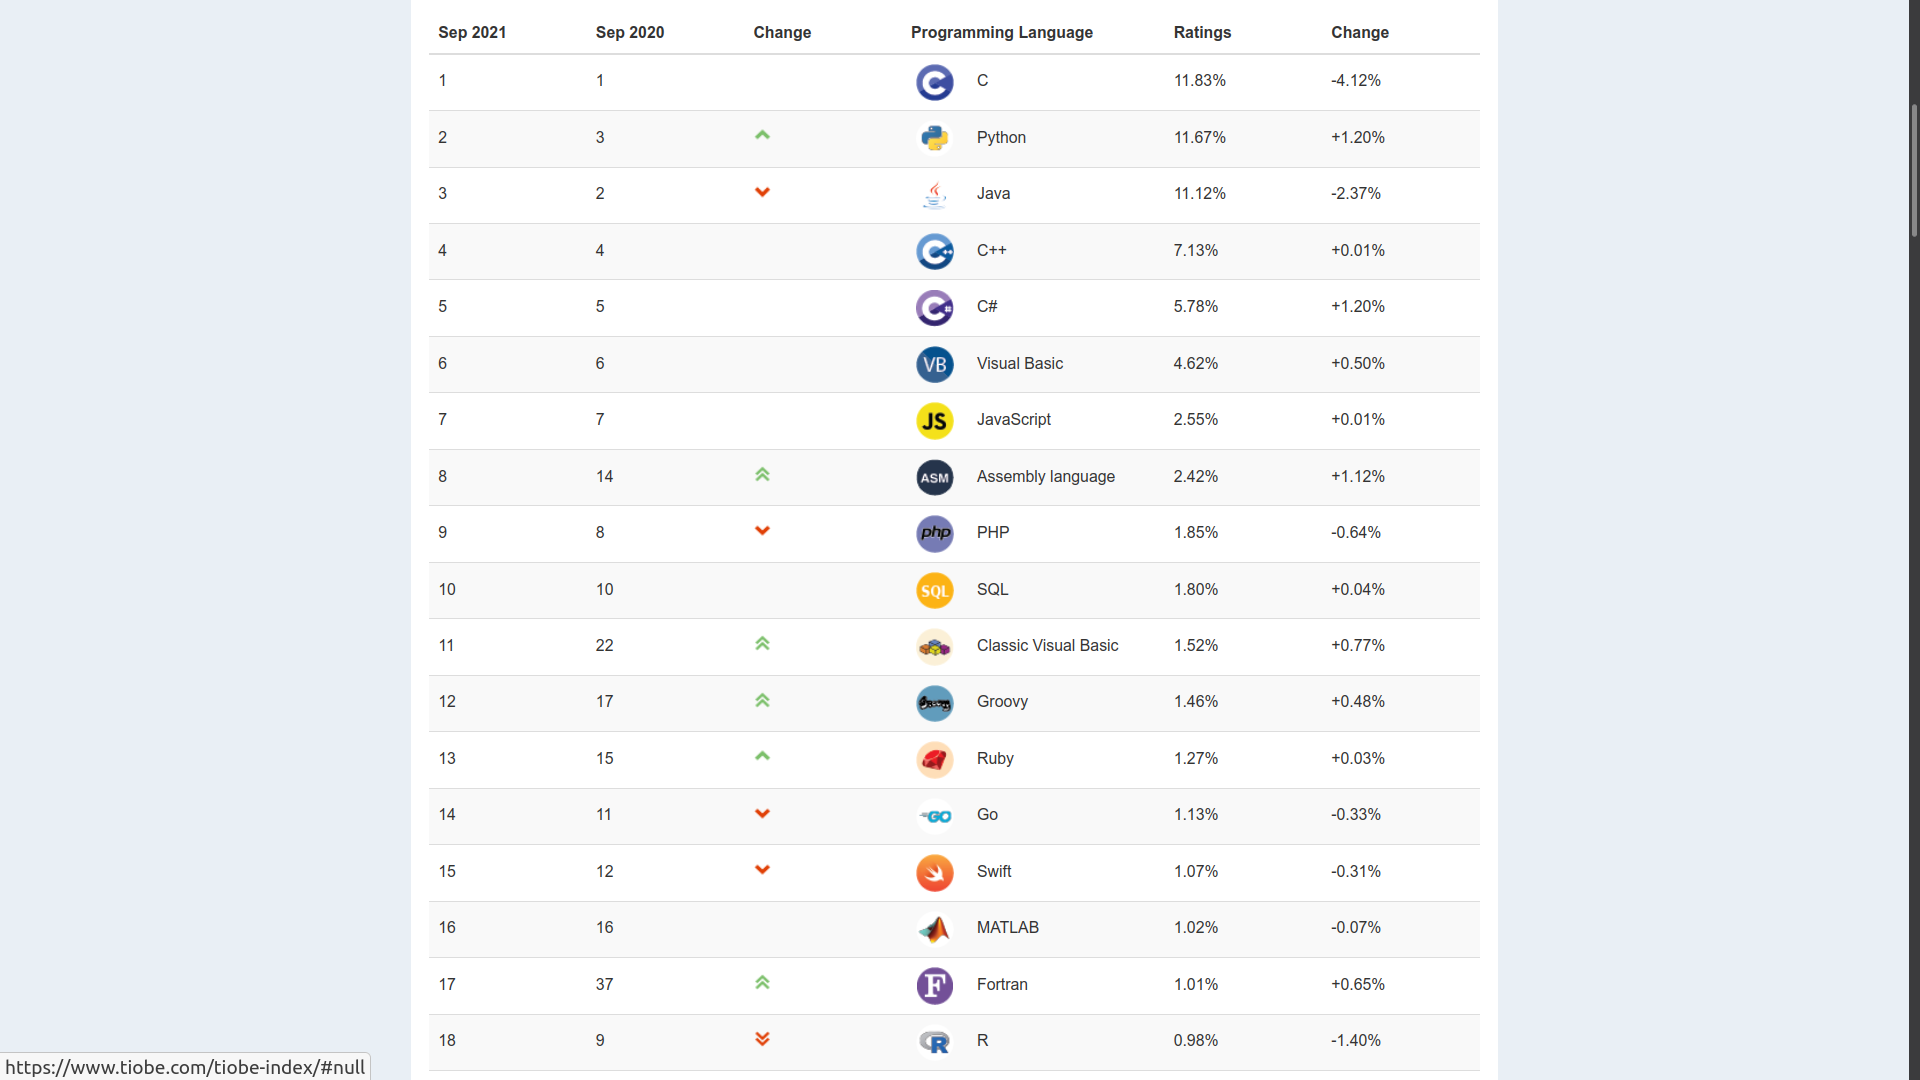
\includegraphics[width=0.9\textwidth]{tiobe2021.png}
  
  \smallskip
  
  \tiny \url{https://www.tiobe.com/tiobe-index/} \normalsize
  
  \smallskip
  
  \begin{itemize}
    \item Besides C of course!
  \end{itemize}
  
\end{frame}



\begin{frame}
  \frametitle{OOP: Classes and Objects}
  
  \begin{itemize}
  \item Basic definitions:
    \begin{itemize}
    \item A \alert{class} is a blueprint for creating objects
    \item An \alert{object} is a concrete realization of a class
    \end{itemize}

  \smallskip
  
  \item You can imagine a class like a project, which is used to
        describe how objects are built and how they works

  \smallskip

  \item You can have multiple objects of the same class
  
  \smallskip
  
  \item The relationship is similar to the one between types and variables:
    \begin{itemize} 
    \item A type is an abstract concept, describing how a variable is
          represented in memory
    \item A variable is a concrete realization of it
    \item You can have several variables of the same type (like several integers
          or several strings)
    \end{itemize}
  
  \smallskip
  
  \item Indeed, to some extent, a class is the generalization of the concept of
        type. It specifies not only how an object \emph{is made} but also how \emph{it behaves}.
  \end{itemize}

\end{frame}


\begin{frame}
  \frametitle{OOP: an example}
  \centering\includegraphics[width=0.2\textwidth]{television.png}
  
  \medskip
  
  \begin{itemize}
  \item Let's consider a familiar object, like a television. It has:
    \smallskip
    \begin{itemize}
    \item A state
      \begin{itemize}
      \item On/off (and possibly standby)
      \item Currently displayed channel
      \item Volume
      \item Brightness, contrast, etc\dots
      \end{itemize}

    \medskip
    
    \item A behaviour
      \smallskip
      \begin{itemize}
      \item Pressing the `power' button will turn ON/OFF
      \item Rotating the volume knob will increase/decrease the volume
      \item Using the buttons on the remote control will change displayed 
            channel, brightness, contrast etc\dots
      \item And don't forget you need to plug-in before use!
      \end{itemize}
    \end{itemize}
  \end{itemize}

\end{frame}


\begin{frame}
  \frametitle{OOP: an example}
 
  \begin{itemize}
    \item How would that be represented in the code?
    \smallskip
      \begin{itemize}
      \item The state can be represented by some \alert{attributes} (variables):
      \begin{itemize}
        \item A boolean can represent the ON/OFF state
        \item For the currently displayed channel you can use an integer
        \item Volume, contrast, luminosity etc\dots they all get their own variable(s)
      \end{itemize}

      \medskip
    
      \item The behaviour can be implemented through the \alert{methods}:
      \smallskip
      \begin{itemize}
        \item For example the turn\_on() and turn\_off() functions may change the value of the variable
              and also produce all the related changes (i.e. start/stop video and audio) 
        \item You will probably have the netx\_channel() and previous\_channel() functions for zapping and so on\dots
        \item Of course it can be much more complex than that!
      \end{itemize}
    \end{itemize}
    
    \medskip
    
    \item Attributes and methods are collectively called \alert{members} of the class
    \medskip
    \item Each object of a specific class is an \alert{instance} of that class
  \end{itemize}

\end{frame}


\begin{frame}
  \frametitle{Python classes}
  \begin{Verbatim}[label=\makebox{\url{https://github.com/lucabaldini/cmepda/tree/master/slides/latex/snippets/class\_tv\_basic.py}},commandchars=\\\{\}]
\PY{c+c1}{\PYZsh{} Here we define the class}
\PY{k}{class} \PY{n+nc}{Television}\PY{p}{:}
    \PY{l+s+sd}{\PYZdq{}\PYZdq{}\PYZdq{} Television class. I will follow the convention of starting class names}
\PY{l+s+sd}{    with an uppercase. \PYZdq{}\PYZdq{}\PYZdq{}}
    \PY{k}{pass} \PY{c+c1}{\PYZsh{} oops we have no code yet!}

\PY{l+s+sd}{\PYZdq{}\PYZdq{}\PYZdq{}To create instances of a class in python we use the parenthesis operator \PYZsq{}()\PYZsq{}.}
\PY{l+s+sd}{The syntax is similar to calling a function \PYZhy{}\PYZhy{} which is actually what is }
\PY{l+s+sd}{happening behind the scenes, as we will see later\PYZdq{}\PYZdq{}\PYZdq{}}
\PY{n}{my\PYZus{}television} \PY{o}{=} \PY{n}{Television}\PY{p}{(}\PY{p}{)} \PY{c+c1}{\PYZsh{} my\PYZus{}television is an instance of the class Television}

\PY{k}{print}\PY{p}{(}\PY{n+nb}{type}\PY{p}{(}\PY{n}{my\PYZus{}television}\PY{p}{)}\PY{p}{)} \PY{c+c1}{\PYZsh{} Check its type}

\PY{n}{your\PYZus{}television} \PY{o}{=} \PY{n}{Television}\PY{p}{(}\PY{p}{)} \PY{c+c1}{\PYZsh{} And this is another instance}

\PY{c+c1}{\PYZsh{} Let\PYZsq{}s check that they are really two different objects}
\PY{k}{print}\PY{p}{(}\PY{n}{my\PYZus{}television} \PY{o+ow}{is} \PY{o+ow}{not} \PY{n}{your\PYZus{}television}\PY{p}{)}

[Output]
<class '__main__.Television'>
True
\end{Verbatim}
\end{frame}


\begin{frame}
  \frametitle{Bonus}
  \framesubtitle{In Python everything is an object of some class!}
  \input{pygments/everything_is_a_class}
\end{frame}


\begin{frame}
  \frametitle{Methods}
  \begin{Verbatim}[label=\makebox{\url{https://github.com/lucabaldini/cmepda/tree/master/slides/latex/snippets/class\_methods.py}},commandchars=\\\{\}]
\PY{k}{class} \PY{n+nc}{Television}\PY{p}{:}
    \PY{l+s+sd}{\PYZdq{}\PYZdq{}\PYZdq{} Class describing a televsion.}
\PY{l+s+sd}{    \PYZdq{}\PYZdq{}\PYZdq{}}
    \PY{k}{def} \PY{n+nf}{turn\PYZus{}on}\PY{p}{(}\PY{n+nb+bp}{self}\PY{p}{,} \PY{n}{channel}\PY{o}{=}\PY{l+m+mi}{1}\PY{p}{)}\PY{p}{:} \PY{c+c1}{\PYZsh{} Class method}
        \PY{l+s+sd}{\PYZdq{}\PYZdq{}\PYZdq{}All the class methods get the object instance as their first argument.}
\PY{l+s+sd}{        It is customary to call this argument \PYZsq{}self\PYZsq{}, though is not required}
\PY{l+s+sd}{        by the language rules (you can call it \PYZsq{}pippo\PYZsq{} and it will work}
\PY{l+s+sd}{        just as well)}
\PY{l+s+sd}{        \PYZdq{}\PYZdq{}\PYZdq{}}
        \PY{n+nb}{print}\PY{p}{(}\PY{l+s+sa}{f}\PY{l+s+s1}{\PYZsq{}}\PY{l+s+s1}{Turning on }\PY{l+s+si}{\PYZob{}}\PY{n+nb+bp}{self}\PY{l+s+si}{\PYZcb{}}\PY{l+s+s1}{\PYZsq{}}\PY{p}{)}
        \PY{n+nb}{print}\PY{p}{(}\PY{l+s+sa}{f}\PY{l+s+s1}{\PYZsq{}}\PY{l+s+s1}{Showing channel }\PY{l+s+si}{\PYZob{}}\PY{n}{channel}\PY{l+s+si}{\PYZcb{}}\PY{l+s+s1}{\PYZsq{}}\PY{p}{)}

\PY{n}{tv} \PY{o}{=} \PY{n}{Television}\PY{p}{(}\PY{p}{)}
\PY{c+c1}{\PYZsh{} Class methods and members are accessed through the \PYZsq{}.\PYZsq{} (dot) operator}
\PY{c+c1}{\PYZsh{} You must not pass the \PYZsq{}self\PYZsq{} argument, it is added automatically!}
\PY{n}{tv}\PY{o}{.}\PY{n}{turn\PYZus{}on}\PY{p}{(}\PY{n}{channel}\PY{o}{=}\PY{l+m+mi}{3}\PY{p}{)}

[Output]
Turning on <__main__.Television object at 0x7f988399d8d0>
Showing channel 3
\end{Verbatim}
\end{frame}


\begin{frame}
  \frametitle{Attributes}
  \begin{Verbatim}[label=\makebox{\url{https://github.com/lucabaldini/cmepda/tree/master/slides/latex/snippets/class\_attributes\_1.py}},commandchars=\\\{\}]
\PY{k}{class} \PY{n+nc}{Television}\PY{p}{:}
    \PY{l+s+sd}{\PYZdq{}\PYZdq{}\PYZdq{} Class describing a televsion.}
\PY{l+s+sd}{    \PYZdq{}\PYZdq{}\PYZdq{}}
    \PY{k}{pass}

\PY{n}{tv} \PY{o}{=} \PY{n}{Television}\PY{p}{(}\PY{p}{)}
\PY{c+c1}{\PYZsh{} Add an attribute manually, with a simple assignment}
\PY{c+c1}{\PYZsh{} Attributes are accessed through the \PYZsq{}.\PYZsq{} (dot) operator}
\PY{n}{tv}\PY{o}{.}\PY{n}{channel} \PY{o}{=} \PY{l+m+mi}{1}
\PY{n+nb}{print} \PY{p}{(}\PY{n}{tv}\PY{o}{.}\PY{n}{channel}\PY{p}{)}
\PY{c+c1}{\PYZsh{} This attribute is not shared with other instances of the class}
\PY{n}{another\PYZus{}tv} \PY{o}{=} \PY{n}{Television}\PY{p}{(}\PY{p}{)}
\PY{n+nb}{print}\PY{p}{(}\PY{n}{another\PYZus{}tv}\PY{o}{.}\PY{n}{channel}\PY{p}{)}

[Output]
1
Traceback (most recent call last):
  File "/home/alberto/computing/cmepda/slides/latex/snippets/class_attributes_1.py", line 13, in <module>
    print(another_tv.channel)
AttributeError: 'Television' object has no attribute 'channel'
\end{Verbatim}
\end{frame}


\begin{frame}
  \frametitle{Attributes}
  \begin{Verbatim}[label=\makebox{\url{https://github.com/lucabaldini/cmepda/tree/master/slides/latex/snippets/class\_attributes\_2.py}},commandchars=\\\{\}]
\PY{k}{class} \PY{n+nc}{Television}\PY{p}{:}
    \PY{l+s+sd}{\PYZdq{}\PYZdq{}\PYZdq{} Class describing a televsion.}
\PY{l+s+sd}{    \PYZdq{}\PYZdq{}\PYZdq{}}
    \PY{n}{NUMBER\PYZus{}OF\PYZus{}CHANNELS} \PY{o}{=} \PY{l+m+mi}{999} \PY{c+c1}{\PYZsh{} This is a class attribute   }
    
\PY{c+c1}{\PYZsh{} We don\PYZsq{}t need an instance to access class attributes}
\PY{k}{print}\PY{p}{(}\PY{n}{Television}\PY{o}{.}\PY{n}{NUMBER\PYZus{}OF\PYZus{}CHANNELS}\PY{p}{)}
\PY{c+c1}{\PYZsh{} But we can also access it through instances}
\PY{n}{tv} \PY{o}{=} \PY{n}{Television}\PY{p}{(}\PY{p}{)}
\PY{k}{print}\PY{p}{(}\PY{n}{tv}\PY{o}{.}\PY{n}{NUMBER\PYZus{}OF\PYZus{}CHANNELS}\PY{p}{)}

\PY{c+c1}{\PYZsh{} Changing the attribute in the class namespace will change it for every instance}
\PY{n}{another\PYZus{}tv} \PY{o}{=} \PY{n}{Television}\PY{p}{(}\PY{p}{)}
\PY{n}{Television}\PY{o}{.}\PY{n}{NUMBER\PYZus{}OF\PYZus{}CHANNELS} \PY{o}{=} \PY{l+m+mi}{998}
\PY{k}{print}\PY{p}{(}\PY{n}{another\PYZus{}tv}\PY{o}{.}\PY{n}{NUMBER\PYZus{}OF\PYZus{}CHANNELS}\PY{p}{)}
\PY{c+c1}{\PYZsh{} But assigning to that attribute in an instance namespace will create a copy!}
\PY{c+c1}{\PYZsh{} Result: the other instances won\PYZsq{}t be affected!}
\PY{n}{tv}\PY{o}{.}\PY{n}{NUMBER\PYZus{}OF\PYZus{}CHANNELS} \PY{o}{=} \PY{l+m+mi}{997}
\PY{k}{print}\PY{p}{(}\PY{n}{another\PYZus{}tv}\PY{o}{.}\PY{n}{NUMBER\PYZus{}OF\PYZus{}CHANNELS}\PY{p}{)}

[Output]
999
999
998
998
\end{Verbatim}
\end{frame}


\begin{frame}
  \frametitle{Constructor}
  
  \begin{itemize}
    \small
    \item Adding attributes like that would be crazy\dots what would happen if I forgot
          to call the 'add\_a\_class\_attribute()' method in the previous example?
    \medskip
    \item Luckily there is a solution for that: the class \alert{constructor}
    \medskip
    \item The constructor is a special method that is called automatically each time
          a class instance is created
    \medskip
    \item A specificity of the constructor is that it cannot return anything
    \medskip
    \item In Python the constructor is the \emph{\_\_init\_\_} method%
          \footnote{Actually the real constructor -- that is the function responsible for 
                    creating the class instances -- is the \emph{\_\_new\_\_} operator, but 99\% of the time you don't need
                    to define that, as all classes have a default one which does the job for you}           
    \medskip
    \item Class methods like \emph{\_\_init\_\_}, with the name surronded by two underscores,
          are called \alert{special} methods or \alert{dunder} methods.
    \medskip
    \item It is good practice to define all your class attributes inside the constructor!

  \end{itemize}

\end{frame}


\begin{frame}
  \frametitle{Constructor}
  \begin{Verbatim}[label=\makebox{\url{https://github.com/lucabaldini/cmepda/tree/master/slides/latex/snippets/class\_constructor.py}},commandchars=\\\{\}]
\PY{k}{class} \PY{n+nc}{Television}\PY{p}{:}
    \PY{l+s+sd}{\PYZdq{}\PYZdq{}\PYZdq{} Class describing a televsion.}
\PY{l+s+sd}{    \PYZdq{}\PYZdq{}\PYZdq{}}
    \PY{k}{def} \PY{n+nf+fm}{\PYZus{}\PYZus{}init\PYZus{}\PYZus{}}\PY{p}{(}\PY{n+nb+bp}{self}\PY{p}{,} \PY{n}{owner}\PY{p}{)}\PY{p}{:}
        \PY{l+s+sd}{\PYZdq{}\PYZdq{}\PYZdq{} The special method \PYZus{}\PYZus{}init\PYZus{}\PYZus{} is called each time a class istance is}
\PY{l+s+sd}{        created.  We can pass arguments to the constructor, just like any}
\PY{l+s+sd}{        function.\PYZdq{}\PYZdq{}\PYZdq{}}
        \PY{n+nb}{print}\PY{p}{(}\PY{l+s+s1}{\PYZsq{}}\PY{l+s+s1}{Creating a television instance...}\PY{l+s+s1}{\PYZsq{}}\PY{p}{)}
        \PY{n+nb+bp}{self}\PY{o}{.}\PY{n}{model} \PY{o}{=} \PY{l+s+s1}{\PYZsq{}}\PY{l+s+s1}{Sv32X\PYZhy{}553T}\PY{l+s+s1}{\PYZsq{}} \PY{c+c1}{\PYZsh{} This class attribute is hard\PYZhy{}coded}
        \PY{n+nb+bp}{self}\PY{o}{.}\PY{n}{owner} \PY{o}{=} \PY{n}{owner} \PY{c+c1}{\PYZsh{} This is set to the value of the argument}

    \PY{k}{def} \PY{n+nf}{print\PYZus{}info}\PY{p}{(}\PY{n+nb+bp}{self}\PY{p}{)}\PY{p}{:}
        \PY{l+s+sd}{\PYZdq{}\PYZdq{}\PYZdq{} Print the model and owner\PYZdq{}\PYZdq{}\PYZdq{}}
        \PY{n+nb}{print}\PY{p}{(}\PY{l+s+sa}{f}\PY{l+s+s1}{\PYZsq{}}\PY{l+s+s1}{This is television model }\PY{l+s+si}{\PYZob{}}\PY{n+nb+bp}{self}\PY{o}{.}\PY{n}{model}\PY{l+s+si}{\PYZcb{}}\PY{l+s+s1}{, owned by }\PY{l+s+si}{\PYZob{}}\PY{n+nb+bp}{self}\PY{o}{.}\PY{n}{owner}\PY{l+s+si}{\PYZcb{}}\PY{l+s+s1}{\PYZsq{}}\PY{p}{)}


\PY{n}{my\PYZus{}television} \PY{o}{=} \PY{n}{Television}\PY{p}{(}\PY{l+s+s1}{\PYZsq{}}\PY{l+s+s1}{Alberto}\PY{l+s+s1}{\PYZsq{}}\PY{p}{)}
\PY{n}{my\PYZus{}television}\PY{o}{.}\PY{n}{print\PYZus{}info}\PY{p}{(}\PY{p}{)}
\PY{n}{batman\PYZus{}television} \PY{o}{=} \PY{n}{Television}\PY{p}{(}\PY{l+s+s1}{\PYZsq{}}\PY{l+s+s1}{Batman}\PY{l+s+s1}{\PYZsq{}}\PY{p}{)}
\PY{n}{batman\PYZus{}television}\PY{o}{.}\PY{n}{print\PYZus{}info}\PY{p}{(}\PY{p}{)}

[Output]
Creating a television instance...
This is television model Sv32X-553T, owned by Alberto
Creating a television instance...
This is television model Sv32X-553T, owned by Batman
\end{Verbatim}
\end{frame}


\begin{frame}
  \frametitle{Digression - namespaces}
  
  \begin{itemize}
    \small
    \item 'Namespaces are one honking great idea -- let's do more of those!'
            (\emph{Tim Peters - The Zen of Python})
    \medskip
    \item A \alert{namespace} in Python is a essentially a dictionary of \emph{unique} names, each one associated to an object (which can be anything: a variable, a function, a class etc\dots)
    \medskip
  \end{itemize}
  
  \centering\includegraphics[width=0.25\textwidth]{types_namespace.png}
  
  \begin{itemize}
    \small
    \item Python creates separate namespaces for many things: for example, each time a function is called a namespace for local variables is created
    \medskip 
    \item You can access objects in the local namespace (and those above -- 
          see picture) just with their name(s); for others you need
          the '.' (dot) operator.
    \medskip
    \item The space of visibility of a variable is called it \alert{scope}.
  \end{itemize}
  
\end{frame}


\begin{frame}
  \frametitle{Instance attributes vs class attributes}
  
  \begin{itemize}
    \small
    \item Each class has a namespace. Plus, each instance of the class get its own additional namespace
    \medskip
    \item The class namespace is automatically visible from each instance namespace, but not the opposite
    \medskip
    \item An attribute in an instance namespace is an \alert{instance attribute}, and cannot be seen or modified
          by other instances of the class
    \medskip
    \item An attribute in the class namespace is a \alert{class attribute} and is shared among all the instances
    \medskip
    \item Since class attributes are not related to a specific instance, they can be accessed without creating one!
    \medskip
    \item Class attributes are useful to set class constants, or default values, or share data among instances 
  \end{itemize}
  
\end{frame}


\begin{frame}
  \frametitle{Class attributes}
  \framesubtitle{(And their strange behaviour)}
  \begin{Verbatim}[label=\makebox{\url{https://github.com/lucabaldini/cmepda/tree/master/slides/latex/snippets/class\_attributes\_3.py}},commandchars=\\\{\}]
\PY{k}{class} \PY{n+nc}{Television}\PY{p}{:}
    \PY{l+s+sd}{\PYZdq{}\PYZdq{}\PYZdq{} Class describing a televsion.}
\PY{l+s+sd}{    \PYZdq{}\PYZdq{}\PYZdq{}}
    \PY{n}{NUMBER\PYZus{}OF\PYZus{}CHANNELS} \PY{o}{=} \PY{l+m+mi}{999} \PY{c+c1}{\PYZsh{} This is a class attribute   }
    
\PY{c+c1}{\PYZsh{} We don\PYZsq{}t need an instance to access class attributes}
\PY{k}{print}\PY{p}{(}\PY{n}{Television}\PY{o}{.}\PY{n}{NUMBER\PYZus{}OF\PYZus{}CHANNELS}\PY{p}{)}
\PY{c+c1}{\PYZsh{} But we can also access it through instances}
\PY{n}{tv} \PY{o}{=} \PY{n}{Television}\PY{p}{(}\PY{p}{)}
\PY{k}{print}\PY{p}{(}\PY{n}{tv}\PY{o}{.}\PY{n}{NUMBER\PYZus{}OF\PYZus{}CHANNELS}\PY{p}{)}

\PY{c+c1}{\PYZsh{} Changing the attribute in the class namespace will change it for every instance}
\PY{n}{another\PYZus{}tv} \PY{o}{=} \PY{n}{Television}\PY{p}{(}\PY{p}{)}
\PY{n}{Television}\PY{o}{.}\PY{n}{NUMBER\PYZus{}OF\PYZus{}CHANNELS} \PY{o}{=} \PY{l+m+mi}{998}
\PY{k}{print}\PY{p}{(}\PY{n}{another\PYZus{}tv}\PY{o}{.}\PY{n}{NUMBER\PYZus{}OF\PYZus{}CHANNELS}\PY{p}{)}
\PY{c+c1}{\PYZsh{} But assigning to that attribute in an instance namespace will create a copy!}
\PY{c+c1}{\PYZsh{} Result: the other instances won\PYZsq{}t be affected!}
\PY{n}{tv}\PY{o}{.}\PY{n}{NUMBER\PYZus{}OF\PYZus{}CHANNELS} \PY{o}{=} \PY{l+m+mi}{997}
\PY{k}{print}\PY{p}{(}\PY{n}{another\PYZus{}tv}\PY{o}{.}\PY{n}{NUMBER\PYZus{}OF\PYZus{}CHANNELS}\PY{p}{)}

[Output]
999
999
998
998
\end{Verbatim}
\end{frame}


\begin{frame}
  \frametitle{Short summary}
  
  \begin{itemize}
    \footnotesize
    \item Object Oriented Programming (OOP) is a widespread programming paradigm,
          supported by many programming languages (old and modern), including Python
    \medskip
    \item An object has a state and a behaviour, represented by member variables (attributes)
          and member functions (methods) respectively
    \medskip
    \item A class is a blueprint for creating objects, each object is an instance of a class
    \medskip
    \item In Python classes are defined with the 'class' keyword and instantiated with the '()' operator
    \medskip
    \item Class attributes and methods (globally called members) are accessed through the '.' operator
    \medskip
    \item All the class methods get the object instance as their first argument (usually named 'self')
    \medskip
    \item You should declare class attributes in the constructor a.k.a. the \emph{\_\_init\_\_} function
    \medskip
    \item Instance attributes are not shared: each instance has its own copy of the data
    \medskip
    \item Class attributes are declared outside methods and are shared among all the instances of a class
  \end{itemize}
  
\end{frame}


\begin{frame}
  \frametitle{Encapsulation - hidden state and interfaces}
  \framesubtitle{Back to the TV example}
  
  \centering\includegraphics[width=0.2\textwidth]{television.png}
  
  \bigskip
  
  \begin{itemize}
  \item Note that part of the state is hidden from the user:
    \begin{itemize}
    \item E.g. internal switches, transistors, etc\dots
    \end{itemize}
  \smallskip
  \item You do not need to know what's going on inside the case to operate a TV!
  \smallskip
  \item All you need to know is how to use the \alert{interface} (the remote
        control, the knobs, the power button, the plug\dots)
  \smallskip
  \item The \alert{implementation} details are hidden: only the TV producer cares about
        them, not the user. 
  \end{itemize}

\end{frame}


\begin{frame}
  \frametitle{Encapsulation}
  
  \begin{itemize}
    \item This leads us to the concept of \alert{encapsulation} 
    \bigskip
    \begin{itemize}
      \item \emph{The state of an object should only be accessed and altered
                  through its publicly exposed interface}
    \end{itemize}
    \bigskip
    \item That way it is easier to find bugs: you know that, if something is wrong
          with an object, the problem lays inside the class code
    \bigskip
    \item That way you can also \emph{enforce behaviour}: for example you can
          prevent from changing the channel if the TV is off
    
  \end{itemize}

\end{frame}


\begin{frame}
  \frametitle{Enforcing behaviour}
  \input{pygments/class_tv_zapping}
\end{frame}


\begin{frame}
  \frametitle{Challenge: how do you get \emph{real} encapsulation?}
  \begin{itemize}
    \item At this point you may be wondering: I can read and modify any class attribute 
          from outside the class using the '.' (dot) operator! 
          Doesn't that break encapsulation?
          
    \bigskip
    
    \item Answer: Yes it does - but there are ways to fix it!
  \end{itemize}
\end{frame}


\begin{frame}
  \frametitle{Pythonic encapsulation}
  
  \begin{itemize}
    \item In languages like C++ you can explicitly declare that some class
          attributes (and methods) are \emph{private}
    \smallskip
    \item In Python there is no concept of \emph{enforced} private attributes
    \smallskip
    \item However, there exists a convention that any attribute/method name prepended by one or two underscore(s) should be considered "private"
    \smallskip
    \item It's like a warning for the class user: you should never access that directly!
    \smallskip
    \item In the case of two underscores Python will actually do a subtle thing to help keeping the data private -- it will 
          prepend \_\emph{classname} to the actual attribute name (see next example)
    \smallskip
    \item However, not everyone in the Python community loves that
    \smallskip
    \item "Never, ever use two leading underscore. This is annoyingly private"\\
           \vspace{0.02\textheight}
           \footnotesize [\emph{Ian Bicking}, creator of pip, virtualenv, and many others]
  \end{itemize}
  
\end{frame}


\begin{frame}
  \frametitle{"Private" attributes in Python}
  \input{pygments/class_tv_private}
\end{frame}


\begin{frame}
  \frametitle{Pythonic encapsulation with properties}
  
  \begin{itemize}
    \item The possibility of making variables "private" (enforced or not) is not enough of course,
          because sometimes we still want to let the user read or even modify the value of the attribute
    \medskip
    \item The "old" solution for that is providing access functions (the infamous "getters/setters")
    \medskip
    \item But the awesome solution is using \alert{properties} (since Python 2.2)
    \medskip
    \item Properties look similar to getters and setters, but with a twist: you keep
          accessing the attribute with the dot operator
    \medskip
    \item In order to understand why this makes a \emph{huge} difference let's 
          start with an example: suppose you have a class for 2-D vectors
  \end{itemize}
  
\end{frame}

\begin{frame}
  \frametitle{Example of a class without encapsulation}
  \begin{Verbatim}[label=\makebox{\url{https://github.com/lucabaldini/cmepda/tree/master/slides/latex/snippets/vector2d\_xy.py}},commandchars=\\\{\}]
\PY{k+kn}{import} \PY{n+nn}{math}

\PY{k}{class} \PY{n+nc}{Vector2d}\PY{p}{:}
    \PY{l+s+sd}{\PYZdq{}\PYZdq{}\PYZdq{} Class representing a Vector2d. We use float() to make sure of storing}
\PY{l+s+sd}{    the coordinates in the correct format \PYZdq{}\PYZdq{}\PYZdq{}}   
    \PY{k}{def} \PY{n+nf+fm}{\PYZus{}\PYZus{}init\PYZus{}\PYZus{}}\PY{p}{(}\PY{n+nb+bp}{self}\PY{p}{,} \PY{n}{x}\PY{p}{,} \PY{n}{y}\PY{p}{)}\PY{p}{:}
        \PY{n+nb+bp}{self}\PY{o}{.}\PY{n}{x} \PY{o}{=} \PY{n+nb}{float}\PY{p}{(}\PY{n}{x}\PY{p}{)}
        \PY{n+nb+bp}{self}\PY{o}{.}\PY{n}{y} \PY{o}{=} \PY{n+nb}{float}\PY{p}{(}\PY{n}{y}\PY{p}{)}
   
    \PY{k}{def} \PY{n+nf}{module}\PY{p}{(}\PY{n+nb+bp}{self}\PY{p}{)}\PY{p}{:}
        \PY{k}{return} \PY{n}{math}\PY{o}{.}\PY{n}{sqrt}\PY{p}{(}\PY{n+nb+bp}{self}\PY{o}{.}\PY{n}{x}\PY{o}{*}\PY{o}{*}\PY{l+m+mi}{2} \PY{o}{+} \PY{n+nb+bp}{self}\PY{o}{.}\PY{n}{y}\PY{o}{*}\PY{o}{*}\PY{l+m+mi}{2}\PY{p}{)}
       
    \PY{k}{def} \PY{n+nf}{angle}\PY{p}{(}\PY{n+nb+bp}{self}\PY{p}{)}\PY{p}{:}
        \PY{k}{return} \PY{n}{math}\PY{o}{.}\PY{n}{atan2}\PY{p}{(}\PY{n+nb+bp}{self}\PY{o}{.}\PY{n}{y}\PY{p}{,} \PY{n+nb+bp}{self}\PY{o}{.}\PY{n}{x}\PY{p}{)}
  
\PY{n}{v} \PY{o}{=} \PY{n}{Vector2d}\PY{p}{(}\PY{l+m+mf}{3.}\PY{p}{,} \PY{o}{\PYZhy{}}\PY{l+m+mf}{1.}\PY{p}{)}
\PY{k}{print}\PY{p}{(}\PY{n}{v}\PY{o}{.}\PY{n}{x}\PY{p}{,} \PY{n}{v}\PY{o}{.}\PY{n}{y}\PY{p}{)}
\PY{k}{print}\PY{p}{(}\PY{n}{v}\PY{o}{.}\PY{n}{module}\PY{p}{(}\PY{p}{)}\PY{p}{,} \PY{n}{v}\PY{o}{.}\PY{n}{angle}\PY{p}{(}\PY{p}{)}\PY{p}{)}

[Output]
3.0 -1.0
3.1622776601683795 -0.3217505543966422
\end{Verbatim}
\end{frame}


\begin{frame}
  \frametitle{Changing your class}
  \begin{itemize}
    \item Suppose you later realize that you use your Vector2d a lot for performing rotations
    \medskip
    \item It would be much faster to store the angle and the module, instead of x and y,
          as the rotation would reduce to a simple addition of the angles
    \medskip
    \item You may think of rewriting your class in that way\dots
  \end{itemize}
\end{frame}


\begin{frame}
  \frametitle{Changing your class}
  \begin{Verbatim}[label=\makebox{\url{https://github.com/lucabaldini/cmepda/tree/master/slides/latex/snippets/vector2d\_rtheta.py}},commandchars=\\\{\}]
\PY{k+kn}{import} \PY{n+nn}{math}

\PY{k}{class} \PY{n+nc}{Vector2d}\PY{p}{:}
    \PY{l+s+sd}{\PYZdq{}\PYZdq{}\PYZdq{} Class representing a Vector2d. We use float() to make sure of storing}
\PY{l+s+sd}{    the coordinates in the correct format \PYZdq{}\PYZdq{}\PYZdq{}}   
    \PY{k}{def} \PY{n+nf+fm}{\PYZus{}\PYZus{}init\PYZus{}\PYZus{}}\PY{p}{(}\PY{n+nb+bp}{self}\PY{p}{,} \PY{n}{module}\PY{p}{,} \PY{n}{angle}\PY{p}{)}\PY{p}{:}
        \PY{n+nb+bp}{self}\PY{o}{.}\PY{n}{module} \PY{o}{=} \PY{n+nb}{float}\PY{p}{(}\PY{n}{module}\PY{p}{)}
        \PY{n+nb+bp}{self}\PY{o}{.}\PY{n}{angle} \PY{o}{=} \PY{n+nb}{float}\PY{p}{(}\PY{n}{angle}\PY{p}{)}
   
    \PY{k}{def} \PY{n+nf}{x}\PY{p}{(}\PY{n+nb+bp}{self}\PY{p}{)}\PY{p}{:}
        \PY{k}{return} \PY{n+nb+bp}{self}\PY{o}{.}\PY{n}{module} \PY{o}{*} \PY{n}{math}\PY{o}{.}\PY{n}{cos}\PY{p}{(}\PY{n+nb+bp}{self}\PY{o}{.}\PY{n}{angle}\PY{p}{)}
       
    \PY{k}{def} \PY{n+nf}{y}\PY{p}{(}\PY{n+nb+bp}{self}\PY{p}{)}\PY{p}{:}
        \PY{k}{return} \PY{n+nb+bp}{self}\PY{o}{.}\PY{n}{module} \PY{o}{*} \PY{n}{math}\PY{o}{.}\PY{n}{sin}\PY{p}{(}\PY{n+nb+bp}{self}\PY{o}{.}\PY{n}{angle}\PY{p}{)}
  
\PY{n}{v} \PY{o}{=} \PY{n}{Vector2d}\PY{p}{(}\PY{l+m+mf}{3.1622776601683795}\PY{p}{,} \PY{o}{\PYZhy{}}\PY{l+m+mf}{0.3217505543966422}\PY{p}{)}
\PY{k}{print}\PY{p}{(}\PY{n}{v}\PY{o}{.}\PY{n}{module}\PY{p}{,} \PY{n}{v}\PY{o}{.}\PY{n}{angle}\PY{p}{)}
\PY{k}{print}\PY{p}{(}\PY{n}{v}\PY{o}{.}\PY{n}{x}\PY{p}{(}\PY{p}{)}\PY{p}{,} \PY{n}{v}\PY{o}{.}\PY{n}{y}\PY{p}{(}\PY{p}{)}\PY{p}{)}

[Output]
3.1622776601683795 -0.3217505543966422
3.0 -1.0
\end{Verbatim}
\end{frame}


\begin{frame}
  \frametitle{The problem}
  \begin{itemize}
    \item \dots now, however, you have a big problem: your old code is broken!
    \medskip
    \item In every place where your were calling \emph{v.x} or \emph{v.module()}
          now you get an error that needs to be fixed
    \medskip
    \item If other people use your code that is even worse, because you are breaking \emph{their} code
    \medskip
    \item Without properties the solution would have been to design the class from
          the start with private attributes and access functions
  \end{itemize}
\end{frame}


\begin{frame}
  \frametitle{Old-style encapsulation: never do that!}
  \begin{Verbatim}[label=\makebox{\url{https://github.com/lucabaldini/cmepda/tree/master/slides/latex/snippets/vector2d\_old\_enc.py}},commandchars=\\\{\}]
\PY{k+kn}{import} \PY{n+nn}{math}

\PY{k}{class} \PY{n+nc}{Vector2d}\PY{p}{:}
    \PY{l+s+sd}{\PYZdq{}\PYZdq{}\PYZdq{} Class representing a Vector2d. Old\PYZhy{}style encapsulation.\PYZdq{}\PYZdq{}\PYZdq{}}   
    \PY{k}{def} \PY{n+nf+fm}{\PYZus{}\PYZus{}init\PYZus{}\PYZus{}}\PY{p}{(}\PY{n+nb+bp}{self}\PY{p}{,} \PY{n}{x}\PY{p}{,} \PY{n}{y}\PY{p}{)}\PY{p}{:}
        \PY{n+nb+bp}{self}\PY{o}{.}\PY{n}{\PYZus{}x} \PY{o}{=} \PY{n+nb}{float}\PY{p}{(}\PY{n}{x}\PY{p}{)}
        \PY{n+nb+bp}{self}\PY{o}{.}\PY{n}{\PYZus{}y} \PY{o}{=} \PY{n+nb}{float}\PY{p}{(}\PY{n}{y}\PY{p}{)}
   
    \PY{k}{def} \PY{n+nf}{x}\PY{p}{(}\PY{n+nb+bp}{self}\PY{p}{)}\PY{p}{:}
        \PY{k}{return} \PY{n+nb+bp}{self}\PY{o}{.}\PY{n}{\PYZus{}x}
       
    \PY{k}{def} \PY{n+nf}{y}\PY{p}{(}\PY{n+nb+bp}{self}\PY{p}{)}\PY{p}{:}
        \PY{k}{return} \PY{n+nb+bp}{self}\PY{o}{.}\PY{n}{\PYZus{}y}
   
    \PY{k}{def} \PY{n+nf}{module}\PY{p}{(}\PY{n+nb+bp}{self}\PY{p}{)}\PY{p}{:}
        \PY{k}{return} \PY{n}{math}\PY{o}{.}\PY{n}{sqrt}\PY{p}{(}\PY{n+nb+bp}{self}\PY{o}{.}\PY{n}{\PYZus{}x}\PY{o}{*}\PY{o}{*}\PY{l+m+mi}{2} \PY{o}{+} \PY{n+nb+bp}{self}\PY{o}{.}\PY{n}{\PYZus{}y}\PY{o}{*}\PY{o}{*}\PY{l+m+mi}{2}\PY{p}{)}
       
    \PY{k}{def} \PY{n+nf}{angle}\PY{p}{(}\PY{n+nb+bp}{self}\PY{p}{)}\PY{p}{:}
        \PY{k}{return} \PY{n}{math}\PY{o}{.}\PY{n}{atan2}\PY{p}{(}\PY{n+nb+bp}{self}\PY{o}{.}\PY{n}{\PYZus{}y}\PY{p}{,} \PY{n+nb+bp}{self}\PY{o}{.}\PY{n}{\PYZus{}x}\PY{p}{)}
  
\PY{n}{v} \PY{o}{=} \PY{n}{Vector2d}\PY{p}{(}\PY{l+m+mf}{3.}\PY{p}{,} \PY{o}{\PYZhy{}}\PY{l+m+mf}{1.}\PY{p}{)}
\PY{k}{print}\PY{p}{(}\PY{n}{v}\PY{o}{.}\PY{n}{x}\PY{p}{(}\PY{p}{)}\PY{p}{,} \PY{n}{v}\PY{o}{.}\PY{n}{y}\PY{p}{(}\PY{p}{)}\PY{p}{)}
\PY{k}{print}\PY{p}{(}\PY{n}{v}\PY{o}{.}\PY{n}{module}\PY{p}{(}\PY{p}{)}\PY{p}{,} \PY{n}{v}\PY{o}{.}\PY{n}{angle}\PY{p}{(}\PY{p}{)}\PY{p}{)}

[Output]
3.0 -1.0
3.1622776601683795 -0.3217505543966422
\end{Verbatim}
\end{frame}

\begin{frame}
\frametitle{Enter properties}
  \begin{itemize}
    \item The class data are now "encapsulated", but that is still not ideal:
    \medskip
    \begin{enumerate}
    \item You have written a lot of code just to provide access to a bunch of
          variables
    \medskip
    \item You will have to write even more methods if you want to let the user
          modify that variables as well (e.g. \emph{set\_x(), set\_y()} and so on)
    \medskip
    \item You have to write all this code right from the start, even if you 
          never need it, otherwise you run the risk of getting screwed later
    \end{enumerate}
    \medskip
    \item \alert{properties} solve the problem by \emph{emulating attributes}
  \end{itemize}
\end{frame}


\begin{frame}
  \frametitle{Properties to emulate attributes}
  \begin{Verbatim}[label=\makebox{\url{https://github.com/lucabaldini/cmepda/tree/master/slides/latex/snippets/vector2d\_property.py}},commandchars=\\\{\}]
\PY{k+kn}{import} \PY{n+nn}{math}

\PY{k}{class} \PY{n+nc}{Vector2d}\PY{p}{:}
    \PY{l+s+sd}{\PYZdq{}\PYZdq{}\PYZdq{} Class representing a Vector2d \PYZhy{} storing module and angle.\PYZdq{}\PYZdq{}\PYZdq{}}   
    \PY{k}{def} \PY{n+nf+fm}{\PYZus{}\PYZus{}init\PYZus{}\PYZus{}}\PY{p}{(}\PY{n+nb+bp}{self}\PY{p}{,} \PY{n}{module}\PY{p}{,} \PY{n}{angle}\PY{p}{)}\PY{p}{:}
        \PY{n+nb+bp}{self}\PY{o}{.}\PY{n}{module} \PY{o}{=} \PY{n+nb}{float}\PY{p}{(}\PY{n}{module}\PY{p}{)}
        \PY{n+nb+bp}{self}\PY{o}{.}\PY{n}{angle} \PY{o}{=} \PY{n+nb}{float}\PY{p}{(}\PY{n}{angle}\PY{p}{)}
   
    \PY{n+nd}{@property}
    \PY{k}{def} \PY{n+nf}{x}\PY{p}{(}\PY{n+nb+bp}{self}\PY{p}{)}\PY{p}{:}
        \PY{k}{return} \PY{n+nb+bp}{self}\PY{o}{.}\PY{n}{module} \PY{o}{*} \PY{n}{math}\PY{o}{.}\PY{n}{cos}\PY{p}{(}\PY{n+nb+bp}{self}\PY{o}{.}\PY{n}{angle}\PY{p}{)}
    
    \PY{n+nd}{@property}
    \PY{k}{def} \PY{n+nf}{y}\PY{p}{(}\PY{n+nb+bp}{self}\PY{p}{)}\PY{p}{:}
        \PY{k}{return} \PY{n+nb+bp}{self}\PY{o}{.}\PY{n}{module} \PY{o}{*} \PY{n}{math}\PY{o}{.}\PY{n}{sin}\PY{p}{(}\PY{n+nb+bp}{self}\PY{o}{.}\PY{n}{angle}\PY{p}{)}
  
\PY{n}{v} \PY{o}{=} \PY{n}{Vector2d}\PY{p}{(}\PY{l+m+mf}{3.1622776601683795}\PY{p}{,} \PY{o}{\PYZhy{}}\PY{l+m+mf}{0.3217505543966422}\PY{p}{)}
\PY{k}{print}\PY{p}{(}\PY{n}{v}\PY{o}{.}\PY{n}{module}\PY{p}{,} \PY{n}{v}\PY{o}{.}\PY{n}{angle}\PY{p}{)}
\PY{c+c1}{\PYZsh{} We don\PYZsq{}t need to call v.x() anymore \PYZhy{} we can simply use v.x!}
\PY{k}{print}\PY{p}{(}\PY{n}{v}\PY{o}{.}\PY{n}{x}\PY{p}{,} \PY{n}{v}\PY{o}{.}\PY{n}{y}\PY{p}{)}

[Output]
3.1622776601683795 -0.3217505543966422
3.0 -1.0
\end{Verbatim}
\end{frame}

\begin{frame}
  \frametitle{Setter properties}
  \begin{Verbatim}[label=\makebox{\url{https://github.com/lucabaldini/cmepda/tree/master/slides/latex/snippets/vector2d\_property\_setter.py}},commandchars=\\\{\}]
\PY{k+kn}{import} \PY{n+nn}{math}

\PY{k}{class} \PY{n+nc}{Vector2d}\PY{p}{:}
    \PY{l+s+sd}{\PYZdq{}\PYZdq{}\PYZdq{} Class representing a Vector2d \PYZhy{} storing module and angle.\PYZdq{}\PYZdq{}\PYZdq{}}   
    \PY{k}{def} \PY{n+nf+fm}{\PYZus{}\PYZus{}init\PYZus{}\PYZus{}}\PY{p}{(}\PY{n+nb+bp}{self}\PY{p}{,} \PY{n}{module}\PY{p}{,} \PY{n}{angle}\PY{p}{)}\PY{p}{:}
        \PY{n+nb+bp}{self}\PY{o}{.}\PY{n}{module} \PY{o}{=} \PY{n+nb}{float}\PY{p}{(}\PY{n}{module}\PY{p}{)}
        \PY{n+nb+bp}{self}\PY{o}{.}\PY{n}{angle} \PY{o}{=} \PY{n+nb}{float}\PY{p}{(}\PY{n}{angle}\PY{p}{)}
   
    \PY{n+nd}{@property}
    \PY{k}{def} \PY{n+nf}{x}\PY{p}{(}\PY{n+nb+bp}{self}\PY{p}{)}\PY{p}{:}
        \PY{k}{return} \PY{n+nb+bp}{self}\PY{o}{.}\PY{n}{module} \PY{o}{*} \PY{n}{math}\PY{o}{.}\PY{n}{cos}\PY{p}{(}\PY{n+nb+bp}{self}\PY{o}{.}\PY{n}{angle}\PY{p}{)}
        
    \PY{n+nd}{@property}
    \PY{k}{def} \PY{n+nf}{y}\PY{p}{(}\PY{n+nb+bp}{self}\PY{p}{)}\PY{p}{:}
        \PY{k}{return} \PY{n+nb+bp}{self}\PY{o}{.}\PY{n}{module} \PY{o}{*} \PY{n}{math}\PY{o}{.}\PY{n}{sin}\PY{p}{(}\PY{n+nb+bp}{self}\PY{o}{.}\PY{n}{angle}\PY{p}{)}
    
    \PY{n+nd}{@x.setter}
    \PY{k}{def} \PY{n+nf}{x}\PY{p}{(}\PY{n+nb+bp}{self}\PY{p}{,} \PY{n}{x}\PY{p}{)}\PY{p}{:} \PY{c+c1}{\PYZsh{} this function must be called as the property}
        \PY{l+s+sd}{\PYZdq{}\PYZdq{}\PYZdq{} Here we actually need to update module and angle\PYZdq{}\PYZdq{}\PYZdq{}}
        \PY{n+nb+bp}{self}\PY{o}{.}\PY{n}{module}\PY{p}{,} \PY{n+nb+bp}{self}\PY{o}{.}\PY{n}{angle} \PY{o}{=} \PY{n}{math}\PY{o}{.}\PY{n}{sqrt}\PY{p}{(}\PY{n}{x}\PY{o}{*}\PY{o}{*}\PY{l+m+mi}{2} \PY{o}{+} \PY{n+nb+bp}{self}\PY{o}{.}\PY{n}{y}\PY{o}{*}\PY{o}{*}\PY{l+m+mi}{2}\PY{p}{)}\PY{p}{,}\PYZbs{}
                                  \PY{n}{math}\PY{o}{.}\PY{n}{atan2}\PY{p}{(}\PY{n+nb+bp}{self}\PY{o}{.}\PY{n}{y}\PY{p}{,} \PY{n}{x}\PY{p}{)}
        
\PY{n}{v} \PY{o}{=} \PY{n}{Vector2d}\PY{p}{(}\PY{l+m+mf}{3.1622776601683795}\PY{p}{,} \PY{o}{\PYZhy{}}\PY{l+m+mf}{0.3217505543966422}\PY{p}{)}
\PY{k}{print}\PY{p}{(}\PY{n}{v}\PY{o}{.}\PY{n}{x}\PY{p}{)}
\PY{n}{v}\PY{o}{.}\PY{n}{x} \PY{o}{=} \PY{l+m+mf}{1.}
\PY{k}{print}\PY{p}{(}\PY{n}{v}\PY{o}{.}\PY{n}{x}\PY{p}{)}

[Output]
3.0
1.0000000000000002
\end{Verbatim}
\end{frame}

\begin{frame}
  \frametitle{Make attributes read-only using properties}
  \begin{Verbatim}[label=\makebox{\url{https://github.com/lucabaldini/cmepda/tree/master/slides/latex/snippets/class\_tv\_encapsulation\_properties.py}},commandchars=\\\{\}]
\PY{k}{class} \PY{n+nc}{Television}\PY{p}{:}
    \PY{l+s+sd}{\PYZdq{}\PYZdq{}\PYZdq{} Class describing a televsion.}
\PY{l+s+sd}{    \PYZdq{}\PYZdq{}\PYZdq{}}
    \PY{k}{def} \PY{n+nf+fm}{\PYZus{}\PYZus{}init\PYZus{}\PYZus{}}\PY{p}{(}\PY{n+nb+bp}{self}\PY{p}{,} \PY{n}{owner}\PY{p}{)}\PY{p}{:}
       \PY{l+s+sd}{\PYZdq{}\PYZdq{}\PYZdq{} Class constructor\PYZdq{}\PYZdq{}\PYZdq{}}
       \PY{n+nb+bp}{self}\PY{o}{.}\PY{n}{\PYZus{}owner} \PY{o}{=} \PY{n}{owner} \PY{c+c1}{\PYZsh{} owner is private}
    
    \PY{n+nd}{@property}
    \PY{k}{def} \PY{n+nf}{owner}\PY{p}{(}\PY{n+nb+bp}{self}\PY{p}{)}\PY{p}{:}
        \PY{k}{return} \PY{n+nb+bp}{self}\PY{o}{.}\PY{n}{\PYZus{}owner}

    \PY{n+nd}{@owner.setter}
    \PY{k}{def} \PY{n+nf}{owner}\PY{p}{(}\PY{n+nb+bp}{self}\PY{p}{,} \PY{n}{new\PYZus{}owner}\PY{p}{)}\PY{p}{:}
       \PY{l+s+sd}{\PYZdq{}\PYZdq{}\PYZdq{} Make the attribute read\PYZhy{}only by acting on the setter\PYZdq{}\PYZdq{}\PYZdq{}}
       \PY{k}{print}\PY{p}{(}\PY{l+s+s1}{\PYZsq{}}\PY{l+s+s1}{Nope \PYZob{}\PYZcb{}. Do you want to steal my tv?}\PY{l+s+s1}{\PYZsq{}}\PY{o}{.}\PY{n}{format}\PY{p}{(}\PY{n}{new\PYZus{}owner}\PY{p}{)}\PY{p}{)}
 
\PY{n}{tv} \PY{o}{=} \PY{n}{Television}\PY{p}{(}\PY{l+s+s1}{\PYZsq{}}\PY{l+s+s1}{Batman}\PY{l+s+s1}{\PYZsq{}}\PY{p}{)}
\PY{k}{print}\PY{p}{(}\PY{l+s+s1}{\PYZsq{}}\PY{l+s+s1}{This tv belongs to \PYZob{}\PYZcb{}}\PY{l+s+s1}{\PYZsq{}}\PY{o}{.}\PY{n}{format}\PY{p}{(}\PY{n}{tv}\PY{o}{.}\PY{n}{owner}\PY{p}{)}\PY{p}{)} 
\PY{n}{tv}\PY{o}{.}\PY{n}{owner} \PY{o}{=} \PY{l+s+s1}{\PYZsq{}}\PY{l+s+s1}{Joker}\PY{l+s+s1}{\PYZsq{}}
\PY{k}{print}\PY{p}{(}\PY{l+s+s1}{\PYZsq{}}\PY{l+s+s1}{This tv belongs to \PYZob{}\PYZcb{}}\PY{l+s+s1}{\PYZsq{}}\PY{o}{.}\PY{n}{format}\PY{p}{(}\PY{n}{tv}\PY{o}{.}\PY{n}{owner}\PY{p}{)}\PY{p}{)}

[Output]
This tv belongs to Batman
Nope Joker. Do you want to steal my tv?
This tv belongs to Batman
\end{Verbatim}
\end{frame}

\begin{frame}
\frametitle{Final note on properties}
  \begin{itemize}
    \item Bottom line: when writing a class, you don't need to make attributes
          private right from the start
    \medskip
    \item You can start with public attributes, and use properties later to
          enforce access/modification rules
    \medskip
    \item That way you only write the code that you really need
  \end{itemize}
\end{frame}

\begin{frame}
  \frametitle{Interface vs implementation mindset}
  \framesubtitle{physicists vs programmers}
  
  \begin{itemize}
    
    \item A physicist thinks:
        
    \medskip
      
    \begin{itemize}
      \item "I have this super-cool algorithm to solve the problem I am working on:
             I will code it carefully, than put together quickly some basic 
             interface to pass data to it and write results to screen / file.
             I need the results quickly for my paper; I can always improve the 
             interface later, right?"
    \end{itemize}
    \medskip
      
    \item A programmer thinks:
    
    \medskip
    
    \begin{itemize}
      \item "I will create a nice interface for the user to handle input/output
             in different formats and I will try to keep it as stable as 
             possible in the future.
             I will start with no algorithm at all -- I will just use random
             numbers to test the interface. I can always implement the
             actual algorithm later, right?"
    \end{itemize}

  \end{itemize}

\end{frame}
 
 
\begin{frame}
  \frametitle{Interfaces}
    
  \begin{itemize}
    \item You don't need to think like a programmer - doing physics is your goal - but
          remember that \alert{interfaces are important}
    \medskip
    \item The concept of interface does not just apply to the program as a whole:
          every significant portion of code (function, class) has its interface
    \medskip
    \item The interface of a class in Python is made by all its "public" members (methods and attributes)
          -- i.e. those without an underscore at the beginning of their name
    \medskip
    \item Changing the interface may break every other piece of code that uses it.
          You want to do that \emph{as less as possible}
    \medskip
    \item You should not access "private" members directly - even if you can. Always
          pass through the interface
    
  \end{itemize}

\end{frame}


\begin{frame}
  \frametitle{Short summary (2)}
    
  \begin{itemize}
    \small
    \item Encapsulation is the technique of hiding part or all the class state to the user; 
          he can only access and modify that through the class methods
    \medskip
    \item Encapsulation helps debugging by limiting the number of places in the code
          that can mutate the state of an object
    \medskip
    \item It can also be useful to enforce behaviour  
    \medskip
    \item Encapsulation in Python is not enforced by the language, but rather relies on conventions
    \medskip
    \item Class members with an underscore at the beginning of their name are
          considered 'private' and should not be accessed directly outside the class
    \smallskip
    \item You can use properties to encapsulate your data at any moment in time - never use 'getters' and 'setters'
    \medskip
    \item Interfaces should not change frequently!
  \end{itemize}
  
\end{frame}


\begin{frame}
  \frametitle{Inheritance}
  \framesubtitle{What and Why}
    
  \begin{itemize}
    \small
    \item Suppose for a moment that you are coding the Monte Carlo for a physics experiment
    \medskip
    \item You want to simulate interactions of charged particles in some detector using OOP paradigm
    \medskip
    \item You may have a class Detetctor and a class for each particle that you need to simulate
    \medskip
    \item Let's say you have a class Electron, a class Positron, a class Proton and a class Alpha
    \medskip
    \item If you think about it, these classes will have a lot of code in common
    \medskip
    \item For example they all need to store their mass, charge, position, velocity (or momentum), possibly spin etc\dots
    \medskip
    \item They may also have similar behaviour, though that is less obvious
    \medskip
    \item We know that duplicate code is evil (DRY): how do we avoid that?
  \end{itemize}
  
\end{frame}


\begin{frame}
  \frametitle{Inerithance}
  \framesubtitle{What and Why}
    
  \begin{itemize}
    \small
    \item Many languages - including Python offer a solution for that: \alert{inheritance}
    \medskip
    \item A class can inherit from another one, automatically obtaining all its functionalities (attributes and methods) and then extending or specializing them
    \medskip
    \item The class which we inherit from is called \emph{Base} class, \emph{Parent} class or (in Python) \emph{Superclass}
    \medskip
    \item The class inheriting is called \emph{Derived} class or \emph{Child} class
    \medskip
    \item In our problem we can imagine to have a base class 'Particle' and many specialized classes inheriting from it
    \medskip
    \item Inheritance is transitive: if class C inherits from class B, and class B inherits from class A, then class C is also a child of class A (and posses all its functionalities)
  \end{itemize}
  
\end{frame}


\begin{frame}
  \frametitle{Inheritance: a basic example}
  \begin{Verbatim}[label=\makebox{\url{https://github.com/lucabaldini/cmepda/tree/master/slides/latex/snippets/inheritance.py}},commandchars=\\\{\}]
\PY{k+kn}{import} \PY{n+nn}{math}

\PY{k}{class} \PY{n+nc}{Particle}\PY{p}{:}
    \PY{l+s+sd}{\PYZdq{}\PYZdq{}\PYZdq{} Class describing a generic particle.}
\PY{l+s+sd}{    \PYZdq{}\PYZdq{}\PYZdq{}}
    \PY{k}{def} \PY{n+nf+fm}{\PYZus{}\PYZus{}init\PYZus{}\PYZus{}}\PY{p}{(}\PY{n+nb+bp}{self}\PY{p}{,} \PY{n}{mass}\PY{p}{,} \PY{n}{charge}\PY{o}{=}\PY{l+m+mi}{0}\PY{p}{,} \PY{n}{name}\PY{o}{=}\PY{k+kc}{None}\PY{p}{,} \PY{n}{momentum}\PY{o}{=}\PY{l+m+mf}{0.}\PY{p}{)}\PY{p}{:}
        \PY{l+s+sd}{\PYZdq{}\PYZdq{}\PYZdq{} Class constructor\PYZdq{}\PYZdq{}\PYZdq{}}
        \PY{n+nb+bp}{self}\PY{o}{.}\PY{n}{mass} \PY{o}{=} \PY{n}{mass} \PY{c+c1}{\PYZsh{} in MeV}
        \PY{n+nb+bp}{self}\PY{o}{.}\PY{n}{charge} \PY{o}{=} \PY{n}{charge} \PY{c+c1}{\PYZsh{} in e}
        \PY{n+nb+bp}{self}\PY{o}{.}\PY{n}{name} \PY{o}{=} \PY{n}{name}
        \PY{n+nb+bp}{self}\PY{o}{.}\PY{n}{momentum} \PY{o}{=} \PY{n}{momentum} \PY{c+c1}{\PYZsh{} in MeV/c}

    \PY{k}{def} \PY{n+nf}{energy}\PY{p}{(}\PY{n+nb+bp}{self}\PY{p}{)}\PY{p}{:}
        \PY{l+s+sd}{\PYZdq{}\PYZdq{}\PYZdq{} Return the energy of the particle in MeV/c\PYZca{}2\PYZdq{}\PYZdq{}\PYZdq{}}
        \PY{k}{return} \PY{n}{math}\PY{o}{.}\PY{n}{sqrt}\PY{p}{(}\PY{n+nb+bp}{self}\PY{o}{.}\PY{n}{momentum}\PY{o}{*}\PY{o}{*}\PY{l+m+mf}{2.} \PY{o}{+} \PY{n+nb+bp}{self}\PY{o}{.}\PY{n}{mass}\PY{o}{*}\PY{o}{*}\PY{l+m+mf}{2.}\PY{p}{)}

\PY{k}{class} \PY{n+nc}{Electron}\PY{p}{(}\PY{n}{Particle}\PY{p}{)}\PY{p}{:}
    \PY{l+s+sd}{\PYZdq{}\PYZdq{}\PYZdq{} Class describing an electron. We inherit from Particle}
\PY{l+s+sd}{    \PYZdq{}\PYZdq{}\PYZdq{}}
    \PY{k}{def} \PY{n+nf+fm}{\PYZus{}\PYZus{}init\PYZus{}\PYZus{}}\PY{p}{(}\PY{n+nb+bp}{self}\PY{p}{,} \PY{n}{momentum}\PY{o}{=}\PY{l+m+mf}{0.}\PY{p}{)}\PY{p}{:}
        \PY{l+s+sd}{\PYZdq{}\PYZdq{}\PYZdq{} Derived class constructor. We call the base class constructor\PYZdq{}\PYZdq{}\PYZdq{}}
        \PY{n}{Particle}\PY{o}{.}\PY{n+nf+fm}{\PYZus{}\PYZus{}init\PYZus{}\PYZus{}}\PY{p}{(}\PY{n+nb+bp}{self}\PY{p}{,} \PY{l+m+mf}{0.511}\PY{p}{,} \PY{o}{\PYZhy{}}\PY{l+m+mf}{1.}\PY{p}{,} \PY{l+s+s1}{\PYZsq{}}\PY{l+s+s1}{e\PYZhy{}}\PY{l+s+s1}{\PYZsq{}}\PY{p}{,} \PY{n}{momentum}\PY{p}{)}

\PY{n}{el} \PY{o}{=} \PY{n}{Electron}\PY{p}{(}\PY{n}{momentum}\PY{o}{=}\PY{l+m+mf}{1.}\PY{p}{)}
\PY{n+nb}{print}\PY{p}{(}\PY{l+s+sa}{f}\PY{l+s+s1}{\PYZsq{}}\PY{l+s+s1}{Energy of }\PY{l+s+si}{\PYZob{}}\PY{n}{el}\PY{o}{.}\PY{n}{name}\PY{l+s+si}{\PYZcb{}}\PY{l+s+s1}{ is }\PY{l+s+si}{\PYZob{}}\PY{n}{el}\PY{o}{.}\PY{n}{energy}\PY{p}{(}\PY{p}{)}\PY{l+s+si}{:}\PY{l+s+s1}{.4f}\PY{l+s+si}{\PYZcb{}}\PY{l+s+s1}{ MeV/c\PYZca{}2}\PY{l+s+s1}{\PYZsq{}}\PY{p}{)}

[Output]
Energy of e- is 1.1230 MeV/c^2
\end{Verbatim}
\end{frame}


\begin{frame}
  \frametitle{Overload}
  \input{pygments/overload}
\end{frame}


\begin{frame}
  \frametitle{Multiple inheritance}
  \begin{Verbatim}[label=\makebox{\url{https://github.com/lucabaldini/cmepda/tree/master/slides/latex/snippets/multiple\_inheritance.py}},commandchars=\\\{\}]
\PY{k}{class} \PY{n+nc}{AudioDevice}\PY{p}{:}
    \PY{k}{def} \PY{n+nf}{play}\PY{p}{(}\PY{n+nb+bp}{self}\PY{p}{,} \PY{n}{channel}\PY{p}{)}\PY{p}{:}
        \PY{n+nb}{print}\PY{p}{(}\PY{l+s+sa}{f}\PY{l+s+s1}{\PYZsq{}}\PY{l+s+s1}{You are listening to channel n. }\PY{l+s+si}{\PYZob{}}\PY{n}{channel}\PY{l+s+si}{\PYZcb{}}\PY{l+s+s1}{\PYZsq{}}\PY{p}{)}

\PY{k}{class} \PY{n+nc}{VideoDevice}\PY{p}{:}
    \PY{k}{def} \PY{n+nf}{play}\PY{p}{(}\PY{n+nb+bp}{self}\PY{p}{,} \PY{n}{channel}\PY{p}{)}\PY{p}{:}
        \PY{n+nb}{print}\PY{p}{(}\PY{l+s+sa}{f}\PY{l+s+s1}{\PYZsq{}}\PY{l+s+s1}{You are looking to channel n. }\PY{l+s+si}{\PYZob{}}\PY{n}{channel}\PY{l+s+si}{\PYZcb{}}\PY{l+s+s1}{\PYZsq{}}\PY{p}{)}

\PY{c+c1}{\PYZsh{} Multiple inheritance!}
\PY{k}{class} \PY{n+nc}{Television}\PY{p}{(}\PY{n}{AudioDevice}\PY{p}{,} \PY{n}{VideoDevice}\PY{p}{)}\PY{p}{:}
    \PY{k}{def} \PY{n+nf}{show}\PY{p}{(}\PY{n+nb+bp}{self}\PY{p}{,} \PY{n}{channel}\PY{p}{)}\PY{p}{:}
        \PY{n}{AudioDevice}\PY{o}{.}\PY{n}{play}\PY{p}{(}\PY{n+nb+bp}{self}\PY{p}{,} \PY{n}{channel}\PY{p}{)}
        \PY{n}{VideoDevice}\PY{o}{.}\PY{n}{play}\PY{p}{(}\PY{n+nb+bp}{self}\PY{p}{,} \PY{n}{channel}\PY{p}{)}

\PY{n}{tv} \PY{o}{=} \PY{n}{Television}\PY{p}{(}\PY{p}{)}
\PY{n}{tv}\PY{o}{.}\PY{n}{show}\PY{p}{(}\PY{l+m+mi}{5}\PY{p}{)}
\PY{c+c1}{\PYZsh{} Is this a good idea?}
\PY{n}{tv}\PY{o}{.}\PY{n}{play}\PY{p}{(}\PY{l+m+mi}{5}\PY{p}{)} \PY{c+c1}{\PYZsh{} Which one do we get? Why?}
\PY{c+c1}{\PYZsh{} Hint}
\PY{c+c1}{\PYZsh{} print(Television.mro())}

[Output]
You are listening to channel n. 5
You are looking to channel n. 5
You are listening to channel n. 5
\end{Verbatim}
\end{frame}


\begin{frame}
  \frametitle{Inerithance}
  \framesubtitle{Infernus Linnaei}
  
  \centering
  \includegraphics[width=0.40\textwidth]{linneo.jpg}~\quad%
  \includegraphics[width=0.55\textwidth]{tassonomy.jpg}
  
  \bigskip
    
  \begin{itemize}
    \item Don't abuse inheritance!
    \medskip
    \item Though bringing order to the World may look appealing\dots
  \end{itemize}
  
\end{frame}


\begin{frame}
  \frametitle{Inherithance}
  \framesubtitle{A real case example}
  
  \centering
  \includegraphics[width=0.8\textwidth]{tk-widgets.png}
   
  \tiny \url{https://wiki.python.org/moin/TkInter} \normalsize
    
  \smallskip
  \begin{itemize}
    \item {\dots}the result may be more complicated than you expect!
  \end{itemize}
\end{frame}


\begin{frame}
  \frametitle{Composition}
    
  \begin{itemize}
    \item \alert{Composition} is a different technique for reusing functionalities
    \medskip
    \item The concept is simple: just use an object of some class as a member of
          a different one
    \medskip
    \item For example we can create the classes 'Engine' and 'Wheel' and than 
          the class 'Car' will have a member of type Engine and 4 members of
          type Wheel
    \medskip
    \item A class like 'Car' in the example is sometimes called an 
          \alert{aggregate} class
  \end{itemize}
  
\end{frame}


\begin{frame}
  \frametitle{Composition}
  \input{pygments/composition}
\end{frame}


\begin{frame}
  \frametitle{Composition vs Inheritance}
    
  \begin{itemize}
    \item Composition models a \alert{'has-a'} relation in the real world: a 
          Car \emph{has} a Engine
    \medskip
    \item Inheritance models a \alert{'is-a'} relation in the real world: an
          Electron \emph{is} a Particle
    \medskip
    \item It may not always be obvious which one to use in your specific case:
          choose wisely!
  \end{itemize}
  
\end{frame}



\begin{frame}
  \frametitle{Pitfalls of Inerithance}
    
  \begin{itemize}
    \item Inheritance is a wild beast. There are entire libraries written about how and when (not) to use it
    
    \bigskip
    
    \item Question for you: should a Square inherits from a Rectangle?
    \item Seems legit: a Square \emph{is} a specialized Rectangle
    \item But what happens if the Rectangle class has a changeHeight() method?
    \bigskip
    
    \bigskip
    
    \item \alert{Liskov Substitution Principle}: you should always be able to use
          a derived class instead of a base class in your code
    \item In other words: a derived class should always extend or specialize
          the functionalities of the base class, never restrict them!
   \end{itemize}
  
\end{frame}



\begin{frame}
  \frametitle{Short summary (3)}
    
  \begin{itemize}
    \item A class can inherit functionalities from one or more other classes (Inheritance)
    \medskip
    \item The class that inherits is call Derived (or Child) class the inherited one is the Base (or Parent) class
    \medskip
    \item Inheritance models an \emph{is-a} relationship
    \medskip
    \item Classes can also incorporate other objects as class members (Composition)
    \medskip
    \item Composition models an \emph{has-a} relationship
    \medskip
    \item Inheritance is tricky: use it with care!
   \end{itemize}
  
\end{frame}



\end{document}
